\documentclass[tikz,border=5pt]{standalone}
\usepackage{pgfplots}
\pgfplotsset{compat=1.18}
\begin{document}
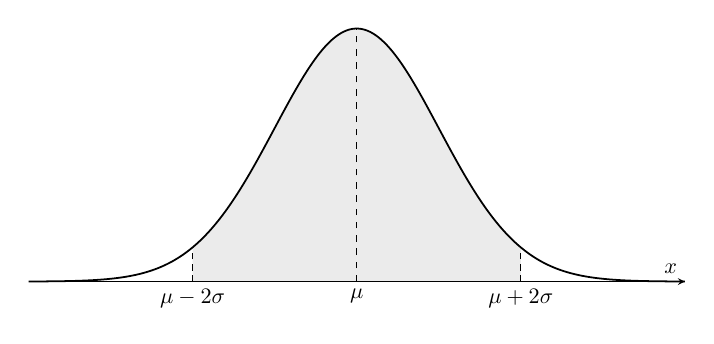
\begin{tikzpicture}[scale=0.8]
  % ----- parameters -----
  \def\muu{0}
  \def\sigmaa{1}

  \begin{axis}[
    axis x line=middle,
    axis y line=none,      % no y-axis
    xmin=\muu-4*\sigmaa, xmax=\muu+4*\sigmaa,
    ymin=0,
    width=12cm, height=6cm,
    xtick=\empty, ytick=\empty,
    xlabel={$x$},
    clip=false
  ]

    % Gaussian curve
    \addplot[thick, domain=\muu-4*\sigmaa:\muu+4*\sigmaa, samples=400]
      {1/(\sigmaa*sqrt(2*pi))*exp(-((x-\muu)^2)/(2*\sigmaa^2))};

    % Shading between muu-2sigma and muu+2sigma (optional)
    \addplot[
      domain=\muu-2*\sigmaa:\muu+2*\sigmaa, samples=200,
      fill=black, fill opacity=0.08, draw=none
    ]
      {1/(\sigmaa*sqrt(2*pi))*exp(-((x-\muu)^2)/(2*\sigmaa^2))}
      \closedcycle;

    % Vertical markers at muu and muu ± 2sigma
    \addplot[dashed] coordinates {(\muu,0) (\muu, {1/(\sigmaa*sqrt(2*pi))})};
    \addplot[densely dashed] coordinates {(\muu-2*\sigmaa,0) (\muu-2*\sigmaa, {1/(\sigmaa*sqrt(2*pi))*exp(-2)})};
    \addplot[densely dashed] coordinates {(\muu+2*\sigmaa,0) (\muu+2*\sigmaa, {1/(\sigmaa*sqrt(2*pi))*exp(-2)})};

    % Labels on x-axis
    \node[below] at (axis cs:\muu,0) {$\mu$};
    \node[below] at (axis cs:\muu-2*\sigmaa,0) {$\mu-2\sigma$};
    \node[below] at (axis cs:\muu+2*\sigmaa,0) {$\mu+2\sigma$};

  \end{axis}
\end{tikzpicture}
\end{document}